Ideally, the score assigned by the model to a decoy should not depend
on its position and orientation.  To allow the model to learn this
invariance, we have randomly sampled the rotational and translational
degrees of freedom of all decoy structures during the training.
%
Figure~\ref{Fig:DecoysScoreDistribution} shows the distributions of
scores for several decoy structures of the same target (T0832),
calculated for 10000??? orientations and positions picked at random.
While the score of a given structure is not strictly invariant under
rotation and translation, it has a relatively narrow, unimodal
distribution.
%%% GL: I'm saying ``unimodal'' instead of ``Gaussian'' because the
%%% distributions of Figure 6 do not appear to be Gaussian.
%G: Got it
More importantly, the difference between the average scores of two
decoys is usually larger than their variances. To reduce the influence
of the choice of orientation and position on the final ranking, we
estimate the score of each decoy from the average of 100 scores
calculated for random rotations and translations.

%%% GL: Figure 5 should go in Supporting information. It's showing a
%%% somewhat minor point (about the effect of rotations versus
%%% translations). Figure 6 tells it all.
%G: I moved this figure to the SI

%%% GL: For consistency, can you show use the same reddish color for
%%% this histogram as the one you use in Figure 6? (for
%%% FALCON_EnvFold_TS1). Also, can you use black lines for the
%%% ``rotations'' histogram?
%G: to do on server

%%% GL: I would remove the Gaussian distribution curve. It's somewhat
%%% of an over-interpretation.
%G: to do on server



\begin{figure}[H]
    \centering
    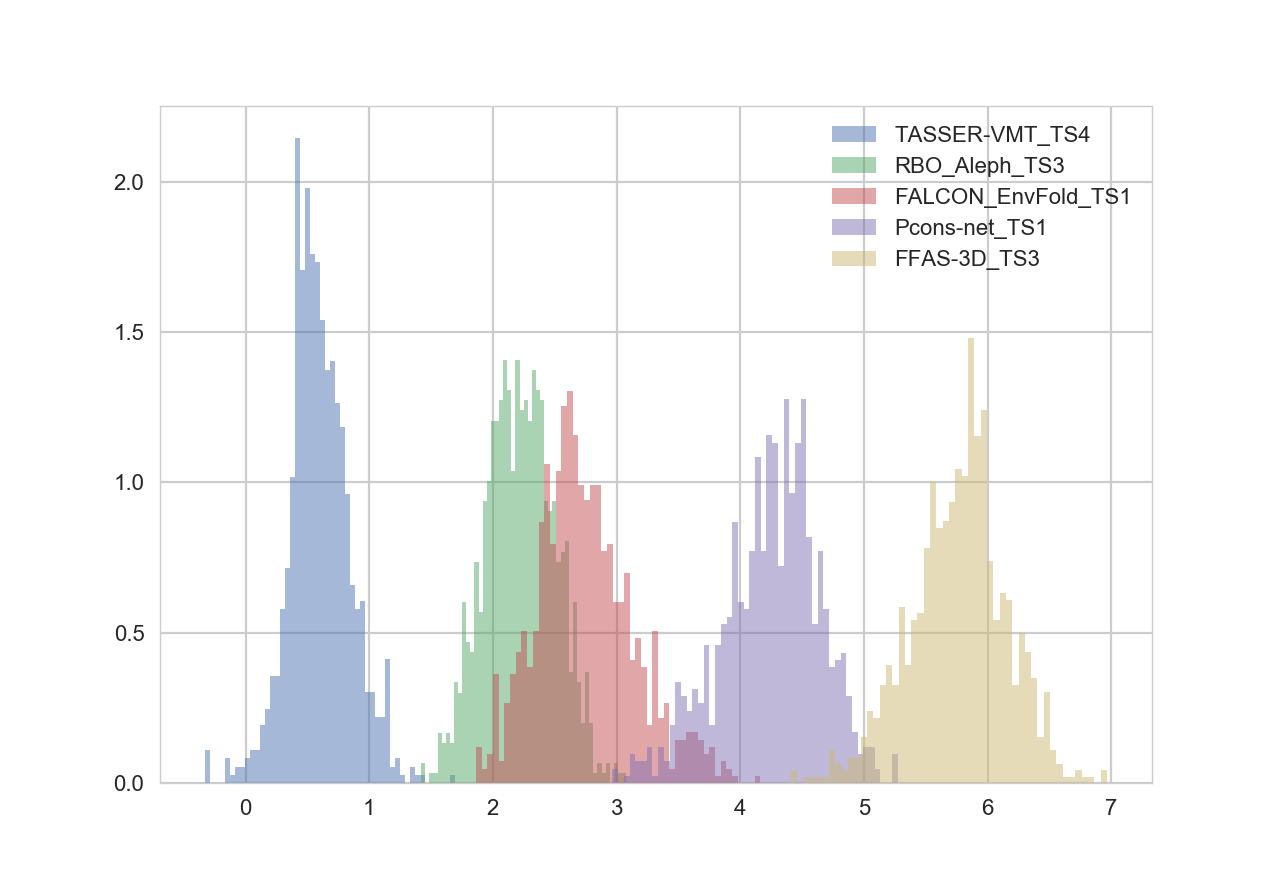
\includegraphics[width=\linewidth]{Fig/decoys_sampling_dist.eps}
%
    \caption{Distributions of the scores of five decoys for target
    T0832 under random translations and rotations. A higher score
    represents a lower quality.}
%
    \label{Fig:DecoysScoreDistribution}
\end{figure}

Table~\ref{Tbl:TestResults} shows a comparison of our model (3DCNN)
with state-of-the-art model quality assessement methods: ProQ2D,
ProQ3D~\cite{uziela2017proq3d}, VoroMQA~\cite{olechnovivc2017voromqa}
and RWPlus~\cite{zhang2010novel}.
ProQ2D uses carefully tuned features based on surface area accessibilities, residue-residue contacts, 
predicted and observed seconday structure, residue conservation and atomic contacts. These features are 
then used as the inputs of deep neural network to predict local and global structure quality. 
ProQ3D employs the same features as ProQ2D as well as Rosetta energy terms based on full-atom and centroid models of the protein. 
This algorithm also uses the features as an input to the deep neural network to predict the 
local and global quality of the candidate structure.
VoroMQA uses knowledge-based potential that depends on the contact surface between two atoms or the solvent. The contact surfaces are calculated 
using Voronoi tesselation and representing atoms as spheres with the radii equal to the Van-der-Waals radii of the corresponding atoms. 
RWPlus is a pairwise knowledge-based potential that uses freely-joined chain model to calculate distance distributions in the reference state.
We chose ProQ2D and ProQ3D as the methods that are derived from the best performing single-model algorithms in CASP11 (ProQ2). The RWPlus 
was selected because it represents previously widespread knowledge-based approach to separate decoys from the corresponding native structures.
VoroMQA was selected, because this approach is rather dissimilar to the common machine-learning techniques and pairwise distance-based scoring potentials.
The other important criterion for selecting these methods is the availability of their source-code or executable. This allowed us to re-evaluate them on 
our CASP11 benchmark, where the decoys side chains were optimized using SCWRL program.

%%% GL: We have to say a few words on each of these methods. What are
%%% they based on? In what sense are they state of the art?
%G: added description of these methods.
%>In what sense are they state of the art?
% This is rather vague question, I wrote why I chose these.


\begin{table}[H]
\begin{center}
\begin{tabular}{ c | c | c | c | c }
    MQA method & Loss & Pearson $R$ & Spearmann $\rho$ & Kendall $\tau$ \\ \hline
    \multicolumn{5}{ c }{Stage 1} \\ \hline
    ProQ3D   &0.048 &0.747 &0.658 &0.516 \\
    ProQ2D   &0.068 &0.722 &0.589 &0.456 \\
    \textbf{3DCNN} &0.071 &0.528 &0.414 &0.318 \\    
    VoroMQA  &0.095 &0.621 &0.504 &0.382 \\
    RWplus   &0.128 &0.500 &0.387 &0.291 \\ \hline
    
    \multicolumn{5}{ c }{Stage 2} \\ \hline
    \textbf{3DCNN} &0.067 &0.420 &0.405 &0.285 \\
    VoroMQA  &0.069 &0.444 &0.437 &0.313 \\ 
    ProQ3D   &0.070 &0.450 &0.429 &0.304 \\
    ProQ2D   &0.077 &0.435 &0.418 &0.296 \\
    RWplus   &0.095 &0.202 &0.246 &0.175 \\ \hline

\end{tabular}
%
    \caption{Performance comparison of our method (3DCNN) with other
    state-of-the-art model quality assessment methods on the CASP11
    dataset stages~1 and 2 (see text). The table reports the absolute,
    per-target average values of the correlation coefficients.}
%%% GL: Is it necessary to mention the order in which the averaging is
%%% done? I thought all targets had the same number of decoys.
%
    \label{Tbl:TestResults}
\end{center}
\end{table}

Figure~\ref{Fig:LossVsECOD} shows how the performance of each
algorithm is affected by the ECOD similarity of the structures used
for testing to those used for training. The test set in broken down
into 5 subsets:
\begin{itemize}
\item
``No information'', the structures for which no ECOD information is
available (T0820, T0823, T0824, T0827, T0835, T0836, and T0838; see
Fig.~\ref{Fig:summaryTable});
\item
``A'', the structures in the same A-group of at least one training
structure but not in the same X-group (T0759, T0763, T0769, etc.);
\item
``A+X'', the structures in the same X-group of at least one training
structure but not in the same H-group (T0760, T0761, T0765, etc.);
\item
``A+X+H+T'', the structures in the same T-group of at least one
training structure but not in the same F-group (T0762, T0766, T0767,
etc.);
\item
``A+X+H+T+F'', the structures in the same F-group of at least one
training structure (T0764, T0768, T0770, etc.).
\end{itemize}
%%% GL: Is this correct?
%
%%% GL: By the way, is Figure 1 correct for structures T0773, T0797,
%%% and T0816?  The ECOD information is available but the structures
%%% belong to A-groups not found in the training set?
%G: to do on server
%
We expect the performance of any knowledge-based MQA method to
increase as the structures used for testing become more similar to the
structures used for training. By contrast, we would expect a purely
first-principles method to show no increase in performance.
%
Both our 3DCNN algorithm and the VoroMQA algorithm show marked
performance gains as proteins become more similar to the training set,
going from an average loss of around $0.10$ for ``no information''
structures to an average loss of around $0.04$ for ``A+X+H+T+F''
structures (see Fig.~\ref{Fig:LossVsECOD}).
%
By comparison, algorithms ProQ2D and ProQ3D show modest performance
gains (if any) and algorithm RWPlus shows a performance independent
from structural similarity.
%
Overall, these results suggest that the 3DCNN and VoroMQA methods make
better use of structural information---and rely more on
memorization---than the ProQ2D, ProQ3D, and RWPlus methods.
%%% GL: Does it make sense?
%G: to do on server


\begin{figure}[H]
    \centering
    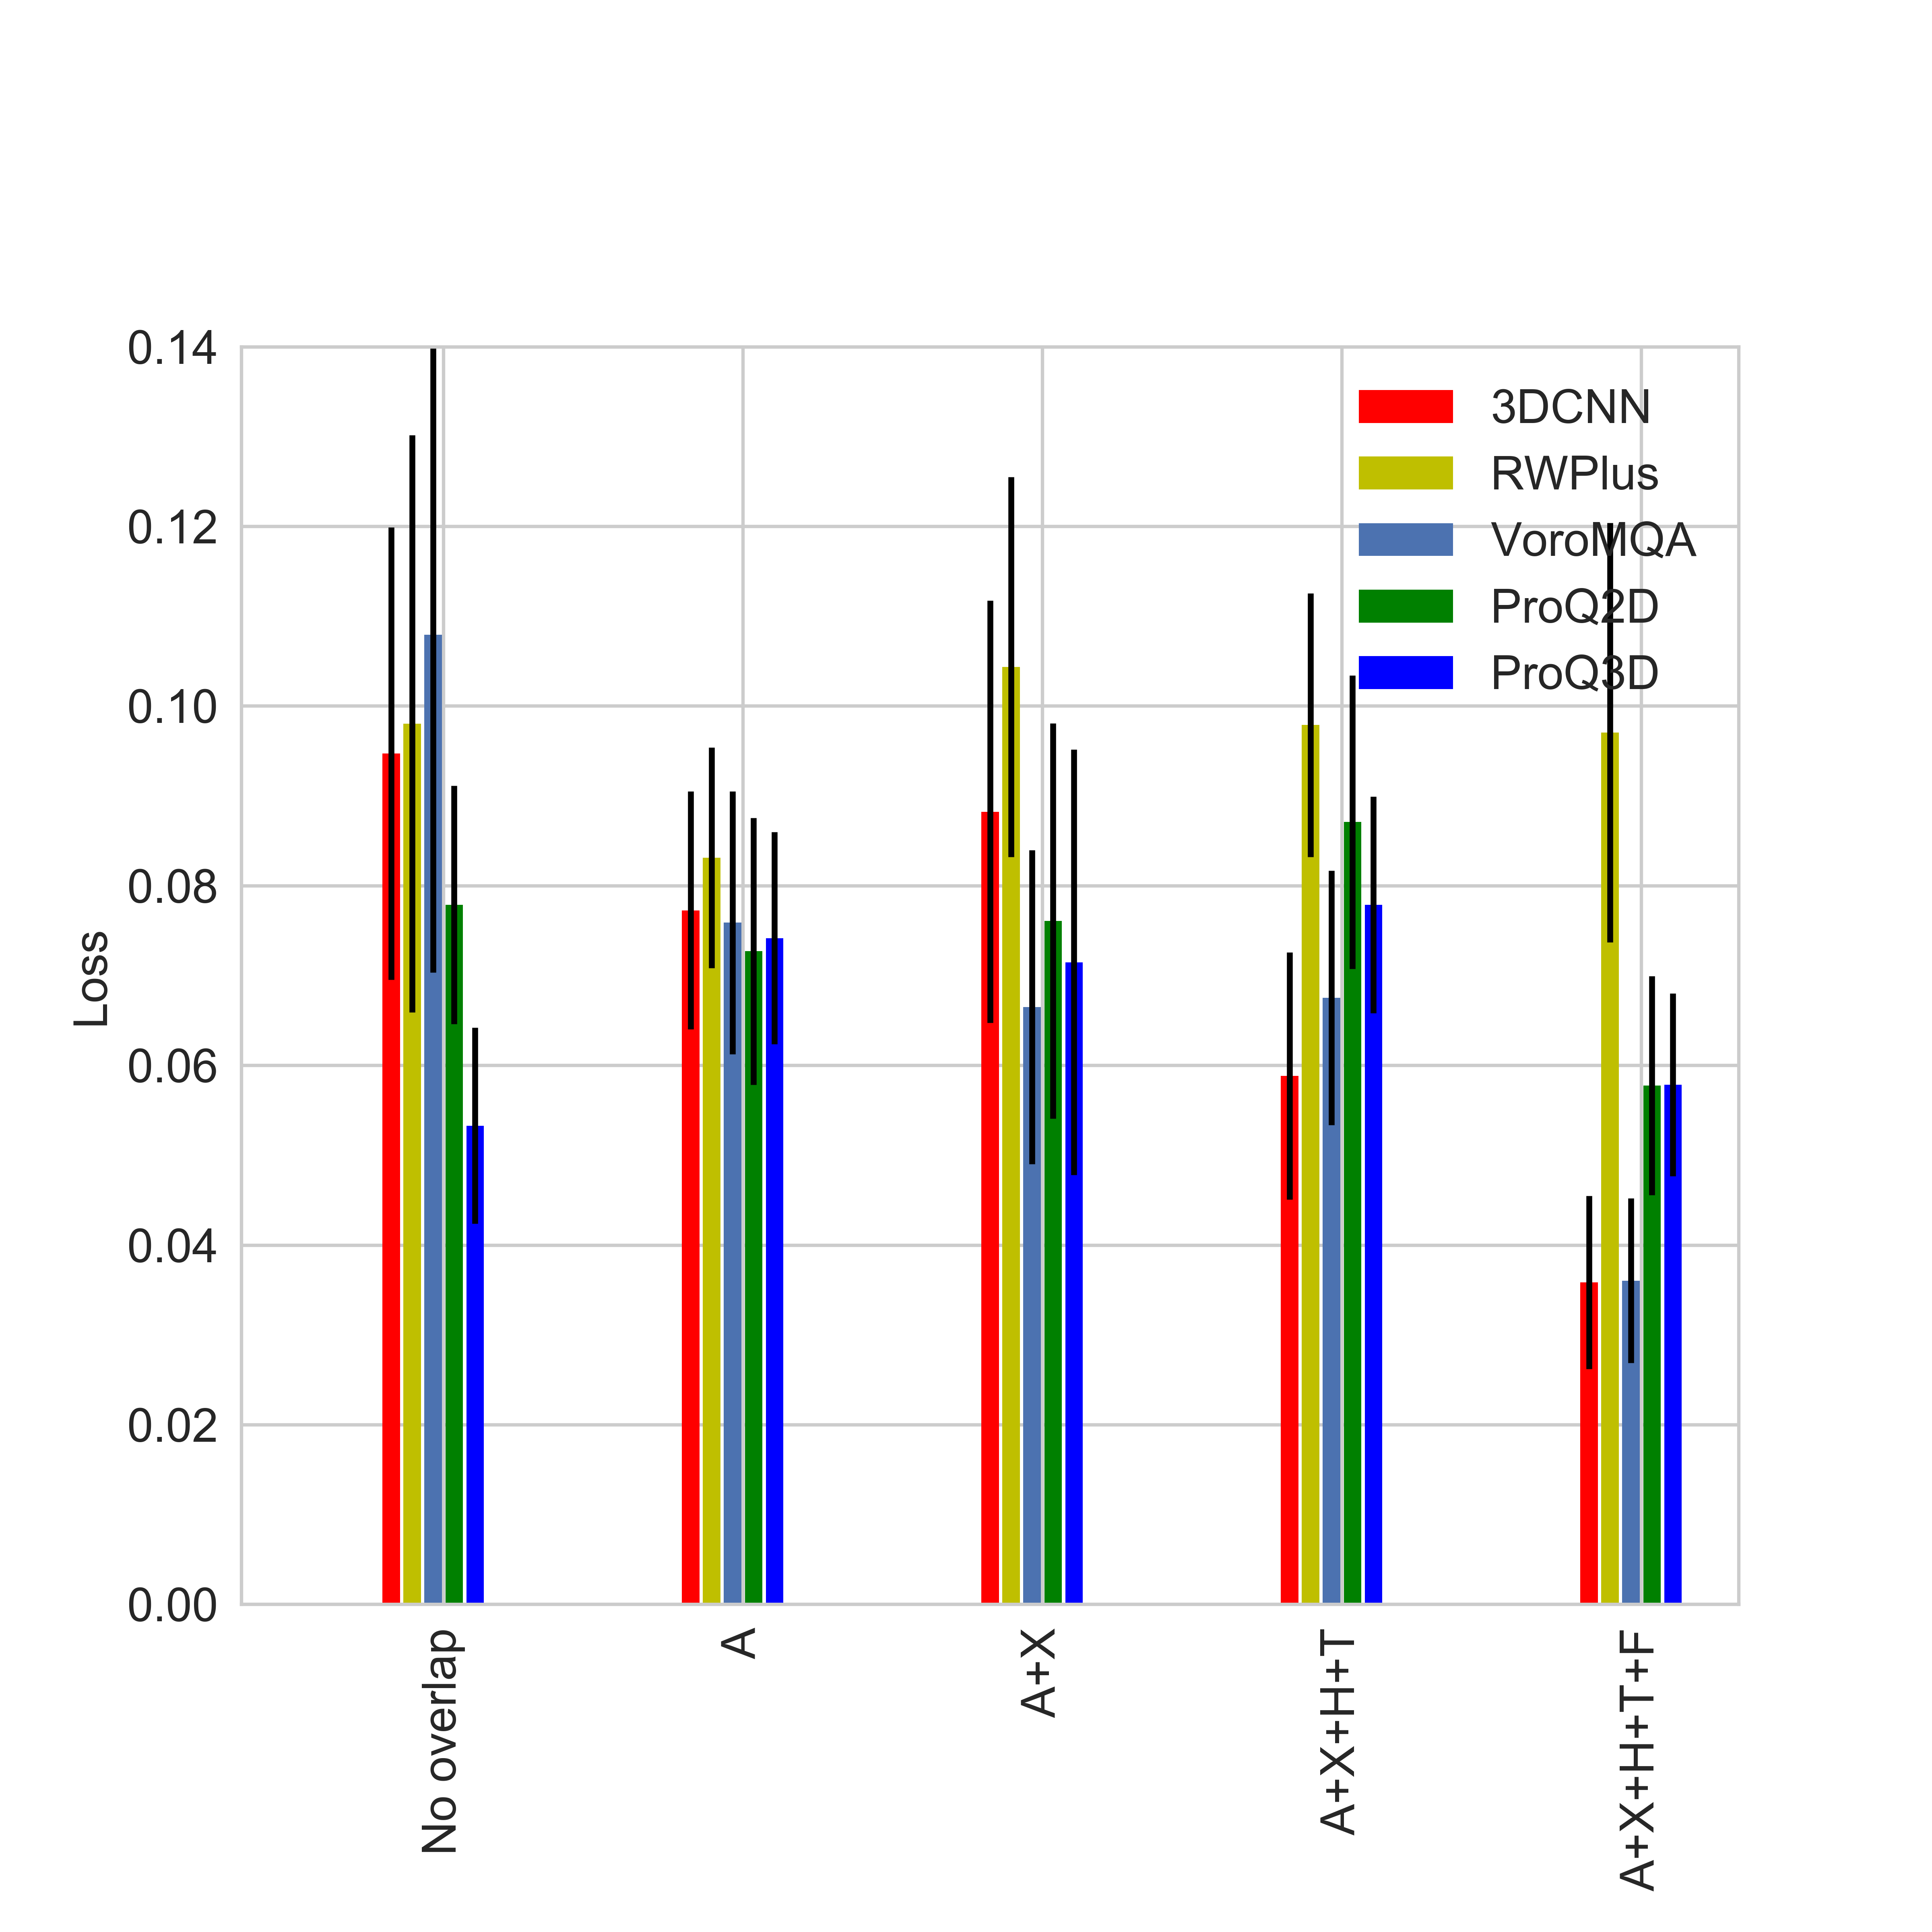
\includegraphics[width=\linewidth]{Fig/LossVsECOD.eps}
%
    \caption{Loss of the MQA algorithms of Table~\ref{Tbl:TestResults}
    on the CASP11 test set stage~2, divided into 5 subsets of
    increasing structural similarity with the training set. The
    subsets are chosen according to the presence in the training set
    of structures belonging to the same ECOD categories (see text for
    details).}
%
    \label{Fig:LossVsECOD}
\end{figure}
